\section{Response Surface Methodology}
\noindent\rule[\linienAbstand]{\linewidth}{\linienDickeDick}

Response surface methodology (RSM) is a statistical technique which is used to model and analyse processes and data in applications in which a response of interest is influenced by several explanatory variables and the aim is to optimise this response.\\
To find the optimum settings of the explanatory variables, it may be useful to proceed in three steps:
\begin{enumerate}
  \item A $2^k$ factorial design (possibly fractional) is used to detect the important influencing factors.
  \item For the most important influencing factors, the main effects are estimated in order to determine the direction of the steepest ascent.
  \item Now we can hope to find the global optimum in the determined direction with a suitabledesign and additional experiments.
\end{enumerate}
This kind of procedure is a response surface exploration which is based on a sequence of experimental design.


\subsection{Response Surface}
\noindent\rule[\linienAbstand]{\linewidth}{\linienDicke}
In the search for relevant influencing factors, we assumed two (or more) levels per factor and used the analysis of variance to estimate and test main effects (and interactions). The model for two factors $A$ and $B$ with two levels each and without interaction is
\begin{equation}
  y_{ij} = \mu_{ij} + \varepsilon_{ij} = \mu + \alpha + \beta_j + \varepsilon_{ij}
\end{equation}

If both explanatory variables $x_1$ and $x_2$ are continuous then the model is
\begin{equation}
  y = f(x_1, x_2) + \varepsilon
\end{equation}
where $\varepsilon$ represents the noise or error observed in the response $y$.
If we denote the expected response by $E(y) = f(x_1, x_2) = \eta$, then the surface represented by
\begin{equation}
  \eta = f(x_1, x_2) + \varepsilon
\end{equation}
is called a response surface.

It is possible to detect deviations (curvature) from the first-order linear model. If no curvature is present and if the plane is a sufficient approximation of the response within the experimental domain, then the mean of the central observations $\bar{y}_c$ and the mean of all the other observations in the $2^k$ factorial design $\bar{y}_f$ are almost the same. If, on the other hand, this difference is significantly different from zero then this is an indication that a model with curvature is more appropriate.\\
The corresponding hypothesis to test the presence of curvature in a 2k design are
\begin{equation}
  \begin{split}
    H_0 &: \;\text{no curvature in the data},\\
    H_1 &: \;\text{curvature in the data}.
  \end{split}
\end{equation}

\begin{figure}[H]
  \centering
  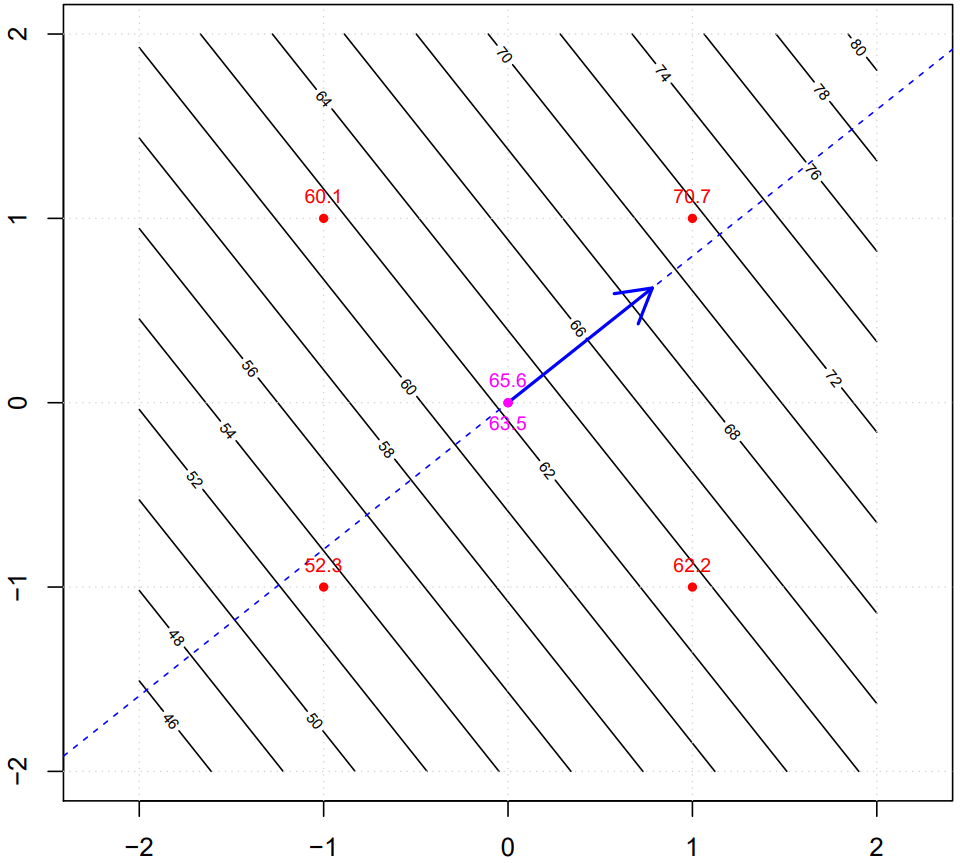
\includegraphics[width=.6\linewidth]{Pics/15.1.2.png}
\end{figure}

Therefore, the test statistic for the curvature in a $2^k$ factorial design is
\begin{equation}
  t_{curve} = \frac{\bar{y}_c -\bar{y}_f}{\sqrt{s_c^2 \left(\frac{1}{n_c} + \frac{1}{2^k}\right)}}
\end{equation}
Under the null hypothesis the test statistic $t_{curv}$ follows a $t$-distribution with $n_c - 1$ degrees of freedom.\\
If the first-order linear model is fits the data well then we can search an optimum along the straight line through the centre of the design and along the estimated gradient.

\subsection{Second-Order Response Surface with Interactions}
\noindent\rule[\linienAbstand]{\linewidth}{\linienDicke}
There are two reasons to use a second-order polynomial:\\
\begin{enumerate}
  \item If we are close to the optimum and the estimated response plane is almost horizontal, i.e. the estimated coefficients are almost zero.\\
  \item If there is curvature in the system, then a polynomial of higher degree must be used, such as the second-order model
\end{enumerate}
\begin{equation}
  y = \beta_0 + \sum_{i=1}^k \beta_i x_i + \sum_{i=1}^k \beta_{ii} x_i^2 + \sum_{i<j} \beta_{ij} x_i x_j + \varepsilon
\end{equation}
In the case of two explanatory variables the model simplifies to
\begin{equation}
  y = \beta_0 + \beta_1 x_1 + \beta_2 x_2 + \beta_{11} x_{21} + \beta_{22}x_{22} + \beta_{12}x_1x_2 + \varepsilon
\end{equation}

The $2^k$ design is not enough to estimate the parameters in the second-order model. To keep the effort within limits, so-called rotatable central composite design or second-order central composite design are used. This design can be obtained from a $2^k$ design by adding more experimental conditions.\\,
For the case of two explanatory variables all experimental conditions in coded variables (except the centre) are equidistant from the center $(0, 0)$. Each factor is measured at five levels. $(+1, -1, +\sqrt{2}, -\sqrt{2}, 0)$
\begin{figure}[H]
  \centering
  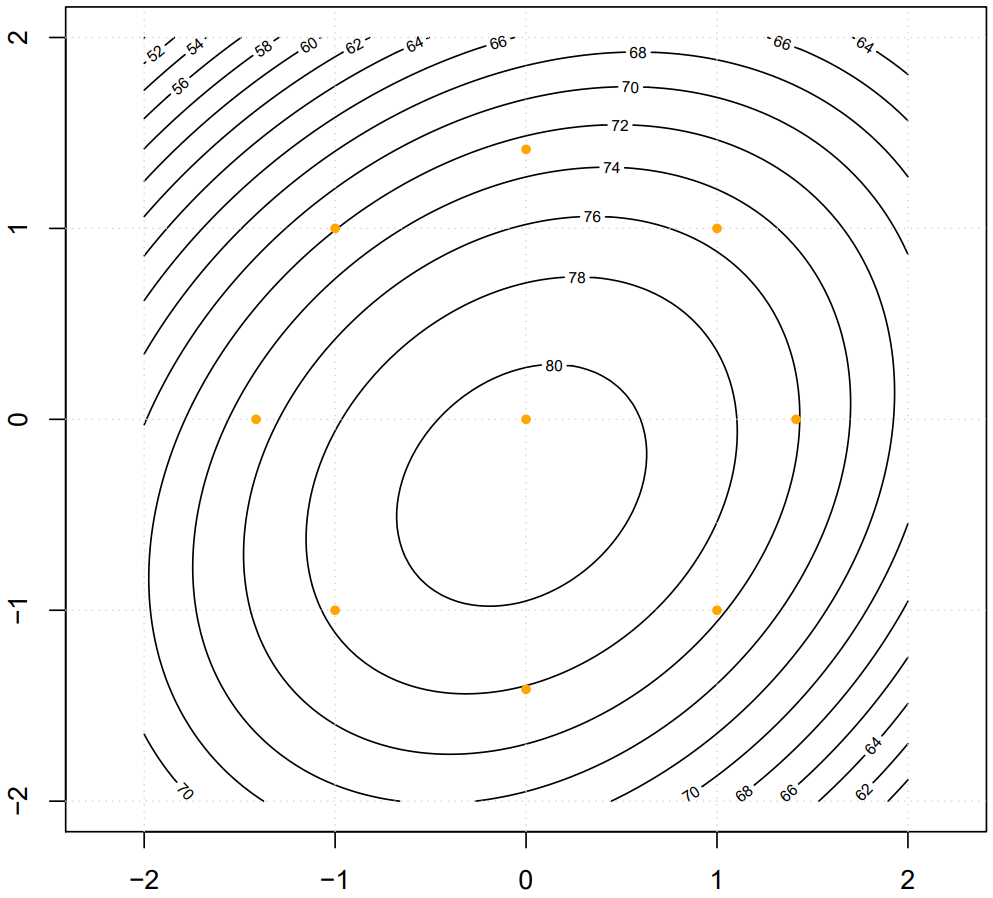
\includegraphics[width=.6\linewidth]{Pics/15.2.1.png}
\end{figure}

\textbf{All experiments in one plot}\\
\begin{figure}[H]
  \centering
  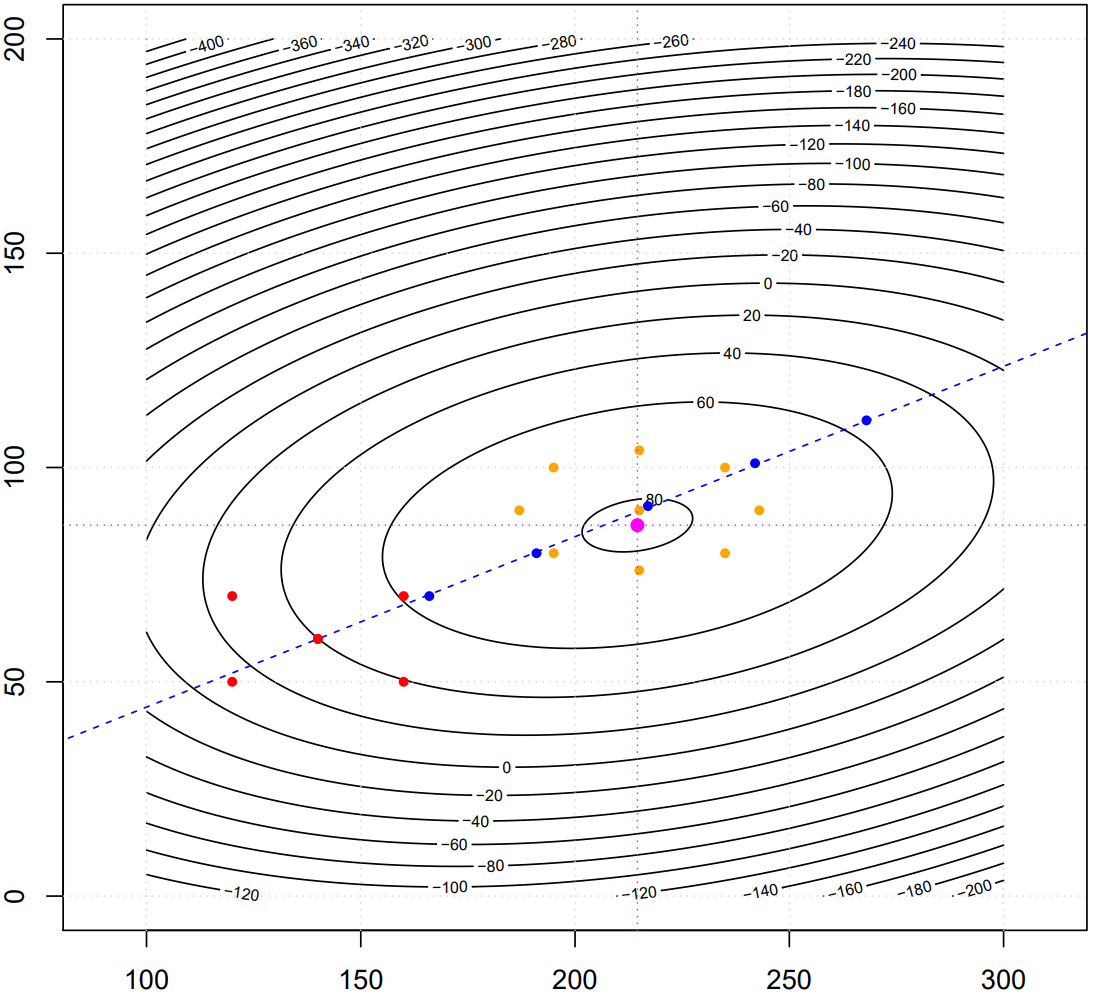
\includegraphics[width=.6\linewidth]{Pics/15.2.3.png}
\end{figure}
Contour plot in original units of the estimated second-order response surface with measurements of the three experiments: Experiment 1 is a $2^2$ factorial design with additional doubled measurement in the centre (red), experiment 2 is an optimisation along the gradient (blue) and experiment 3 is a rotatable central composite design (orange). Optimal settings (magenta).
